\documentclass[journal,12pt,twocolumn]{IEEEtran}

\usepackage{setspace}
\usepackage{gensymb}

\singlespacing


\usepackage[cmex10]{amsmath}

\usepackage{amsthm}

\usepackage{mathrsfs}
\usepackage{txfonts}
\usepackage{stfloats}
\usepackage{bm}
\usepackage{cite}
\usepackage{cases}
\usepackage{subfig}

\usepackage{longtable}
\usepackage{multirow}

\usepackage{enumitem}
\usepackage{mathtools}
\usepackage{steinmetz}
\usepackage{tikz}
\usepackage{circuitikz}
\usepackage{verbatim}
\usepackage{tfrupee}
\usepackage[breaklinks=true]{hyperref}
\usepackage{graphicx}
\usepackage{tkz-euclide}
\usepackage{float}

\usetikzlibrary{calc,math}
\usepackage{listings}
\usepackage{color} %%
\usepackage{array} %%
\usepackage{longtable} %%
\usepackage{calc} %%
\usepackage{multirow} %%
\usepackage{hhline} %%
\usepackage{ifthen} %%
\usepackage{lscape}
\usepackage{multicol}
\usepackage{chngcntr}

\DeclareMathOperator*{\Res}{Res}

\renewcommand\thesection{\arabic{section}}
\renewcommand\thesubsection{\thesection.\arabic{subsection}}
\renewcommand\thesubsubsection{\thesubsection.\arabic{subsubsection}}

\renewcommand\thesectiondis{\arabic{section}}
\renewcommand\thesubsectiondis{\thesectiondis.\arabic{subsection}}
\renewcommand\thesubsubsectiondis{\thesubsectiondis.\arabic{subsubsection}}


\hyphenation{op-tical net-works semi-conduc-tor}
\def\inputGnumericTable{} %%

\lstset{
%language=C,
frame=single,
breaklines=true,
columns=fullflexible
}
\begin{document}


\newtheorem{theorem}{Theorem}[section]
\newtheorem{problem}{Problem}
\newtheorem{proposition}{Proposition}[section]
\newtheorem{lemma}{Lemma}[section]
\newtheorem{corollary}[theorem]{Corollary}
\newtheorem{example}{Example}[section]
\newtheorem{definition}[problem]{Definition}

\newcommand{\BEQA}{\begin{eqnarray}}
\newcommand{\EEQA}{\end{eqnarray}}
\newcommand{\define}{\stackrel{\triangle}{=}}
\bibliographystyle{IEEEtran}
\providecommand{\mbf}{\mathbf}
\providecommand{\pr}[1]{\ensuremath{\Pr\left(#1\right)}}
\providecommand{\qfunc}[1]{\ensuremath{Q\left(#1\right)}}
\providecommand{\sbrak}[1]{\ensuremath{{}\left[#1\right]}}
\providecommand{\lsbrak}[1]{\ensuremath{{}\left[#1\right.}}
\providecommand{\rsbrak}[1]{\ensuremath{{}\left.#1\right]}}
\providecommand{\brak}[1]{\ensuremath{\left(#1\right)}}
\providecommand{\lbrak}[1]{\ensuremath{\left(#1\right.}}
\providecommand{\rbrak}[1]{\ensuremath{\left.#1\right)}}
\providecommand{\cbrak}[1]{\ensuremath{\left\{#1\right\}}}
\providecommand{\lcbrak}[1]{\ensuremath{\left\{#1\right.}}
\providecommand{\rcbrak}[1]{\ensuremath{\left.#1\right\}}}
\theoremstyle{remark}
\newtheorem{rem}{Remark}
\newcommand{\sgn}{\mathop{\mathrm{sgn}}}
\providecommand{\abs}[1]{\left\vert#1\right\vert}
\providecommand{\res}[1]{\Res\displaylimits_{#1}}
\providecommand{\norm}[1]{\left\lVert#1\right\rVert}
%\providecommand{\norm}[1]{\lVert#1\rVert}
\providecommand{\mtx}[1]{\mathbf{#1}}
\providecommand{\mean}[1]{E\left[ #1 \right]}
\providecommand{\fourier}{\overset{\mathcal{F}}{ \rightleftharpoons}}
%\providecommand{\hilbert}{\overset{\mathcal{H}}{ \rightleftharpoons}}
\providecommand{\system}{\overset{\mathcal{H}}{ \longleftrightarrow}}
%\newcommand{\solution}[2]{\textbf{Solution:}{#1}}
\newcommand{\solution}{\noindent \textbf{Solution: }}
\newcommand{\cosec}{\,\text{cosec}\,}
\providecommand{\dec}[2]{\ensuremath{\overset{#1}{\underset{#2}{\gtrless}}}}
\newcommand{\myvec}[1]{\ensuremath{\begin{pmatrix}#1\end{pmatrix}}}
\newcommand{\mydet}[1]{\ensuremath{\begin{vmatrix}#1\end{vmatrix}}}
\numberwithin{equation}{subsection}
\makeatletter
\@addtoreset{figure}{problem}
\makeatother
\let\StandardTheFigure\thefigure
\let\vec\mathbf
\renewcommand{\thefigure}{\theproblem}
\def\putbox#1#2#3{\makebox[0in][l]{\makebox[#1][l]{}\raisebox{\baselineskip}[0in][0in]{\raisebox{#2}[0in][0in]{#3}}}}
\def\rightbox#1{\makebox[0in][r]{#1}}
\def\centbox#1{\makebox[0in]{#1}}
\def\topbox#1{\raisebox{-\baselineskip}[0in][0in]{#1}}
\def\midbox#1{\raisebox{-0.5\baselineskip}[0in][0in]{#1}}
\vspace{3cm}
\title{Assignment No.7}
\author{Valli Devi Bolla}
\maketitle
\newpage
\bigskip
\renewcommand{\thefigure}{\theenumi}
\renewcommand{\thetable}{\theenumi}
Download all python codes from
\begin{lstlisting}
https://github.com/Vallidevibolla/Assignment-7/blob/main/code.py
\end{lstlisting}
%
and latex-tikz codes from
%
\begin{lstlisting}
https://github.com/Vallidevibolla/Assignment-7/blob/main/main.tex
\end{lstlisting}
%
Question taken from
\begin{lstlisting}
https://github.com/gadepall/ncert/blob/main/linalg/optimization/gvv_ncert_opt.pdf-Q.no.2.11
\end{lstlisting}
%
%https://github.com/gadepall/ncert/blob/main/linalg/optimization/solutions/4/5/Code/Assignment_3.py
%
\section{Question 2.11}
Maximise
\begin{align}
Z = x + y  
\end{align}
subject to
\begin{align}
x-y \leq -1 \\
x+y \leq 0 \\
x \succeq 0
y \succeq 0
\end{align}
\section{Solution}
\begin{align}
Z=x+y\\
x-y=-1\\
-x+y=0
\end{align}
We will write the matrix forms
\begin{align}
\myvec{1 & -1 & -1 \\ 1 & 1 & 0}
\end{align}
By using RREF method we will get 

\begin{align}
\myvec{1 & -1 & -1 \\ 1 & 1 & 0}
\xleftrightarrow{R_2\rightarrow R_2-R_1}
\myvec{1 & -1 & -1 \\ 0 & 2 & 1}\\
\xleftrightarrow{R_2\rightarrow \frac{R_2}{2}}
\myvec{1 & -1 & -1 \\ 0 & 1 & \frac{1}{2}}
\xleftrightarrow{R_2\rightarrow R_2+R_1}
\myvec{1 & 0 & \frac{-1}{2} \\ 0 & 1 & \frac{1}{2}}
\end{align}

\begin{align}
\vec{x}= \frac{-1}{2}\\
\vec{y}= \frac{1}{2}
\end{align}
We have determined the optimal solution to be:
\begin{align}
(x,y)=\left(\frac{-1}{2},\frac{1}{2}\right)\\
Z=x+y\\
Z=\frac{-1}{2}+\frac{1}{2}\\
Z=0
\end{align}

The given problem can be expressed in general as matrix inequality as:
%\begin{align}
%\max_{\vec{x}} Z &= \myvec{1 & 1}\vec{x}
%\\
%s.t. \quad 
%\myvec{
%1 & -1
%\\
%-1 & 1
%}
%\vec{x} &\preceq \myvec{-1\\0}
%\\
%\vec{x} &\succeq \vec{0}\\
%\vec{y} &\succeq \vec{0}
%\end{align}
\begin{align}
\max_{\vec{x}} &\vec{c}^{T}\vec{x}
\\
s.t. \quad \vec{A}\vec{x} &\le \vec{b},
\\
\vec{x} &\succeq\vec{0}\\
\vec{y} &\succeq \vec{0}
\end{align}
%
where
\begin{align}
\vec{c} &= \myvec{-1 \\ -1}
\\
\vec{A} &=
\myvec{
1 & -1
\\
1 & 1
}
\\
\vec{b}&=\myvec{-1\\0}
%
\end{align}
%
and can be solved using {\em cvxpy}. 
Hence,
\begin{align}
\vec{x} = \myvec{-0.5\\0.5}, Z = 0
\end{align}


\begin{figure}[ht]
    \centering
    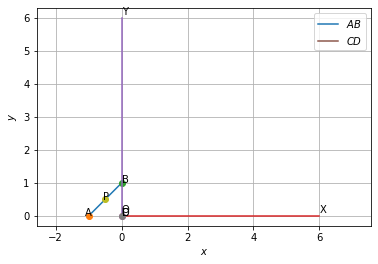
\includegraphics[width=\columnwidth]{download.png}
    \caption{Graphical solution}
    \label{Graphical solution}
\end{figure}

\end{document}
